\section{Accessibilit�}
Durante la progettazione si � sempre cercato di garantire l'accessibilit� a tutte le categorie di utenti seguendo le linee guida WAI.\vspace{-0.2cm}
\subsection{Colori}
Per migliorare l'accessibili� al sito si � evitato di utilizzare combinazioni di colori che potessero creare problemi di accessibilit�, usabilit� e comprensione del contenuto a persone affette da daltonismo. Si riportano di seguito degli screenshot di varie simulazioni di daltonismo della pagina Attivit�.\\
\begin{figure}[h]
	\centering
	\subfloat[][\emph{Immagine Originale}]
	{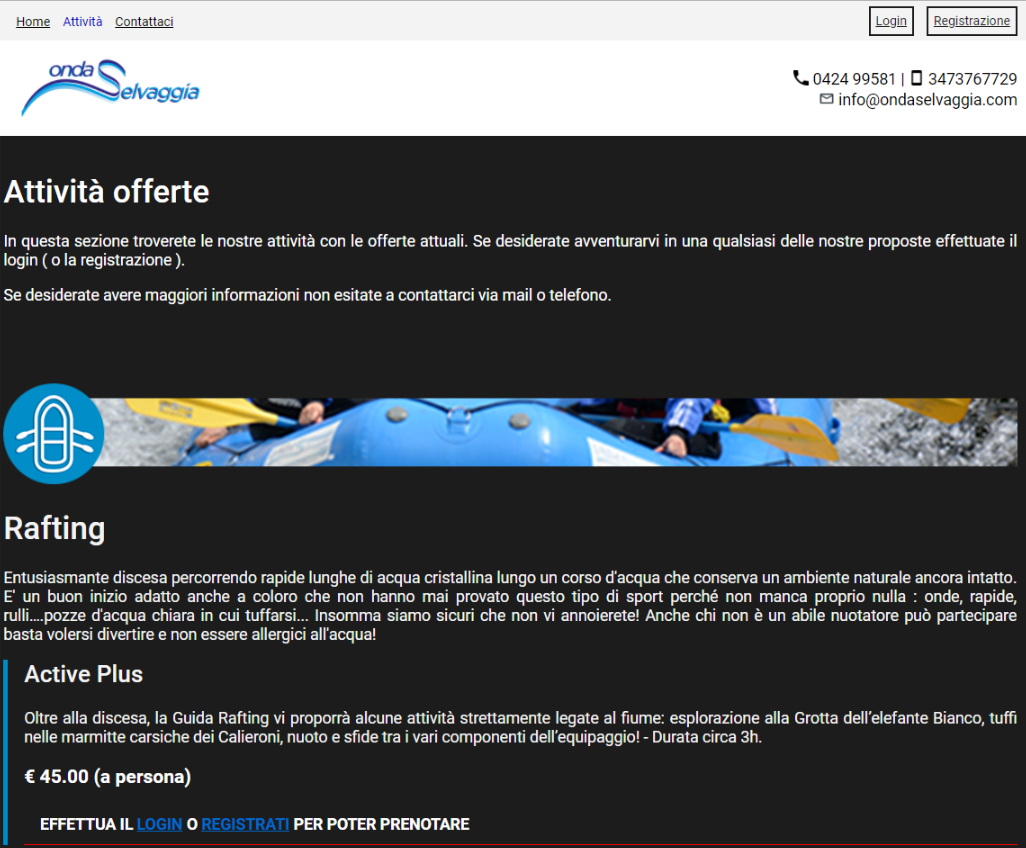
\includegraphics[scale=0.26]{images/normal_color.png}} \quad
	\subfloat[][\emph{Deutenatropia}]
	{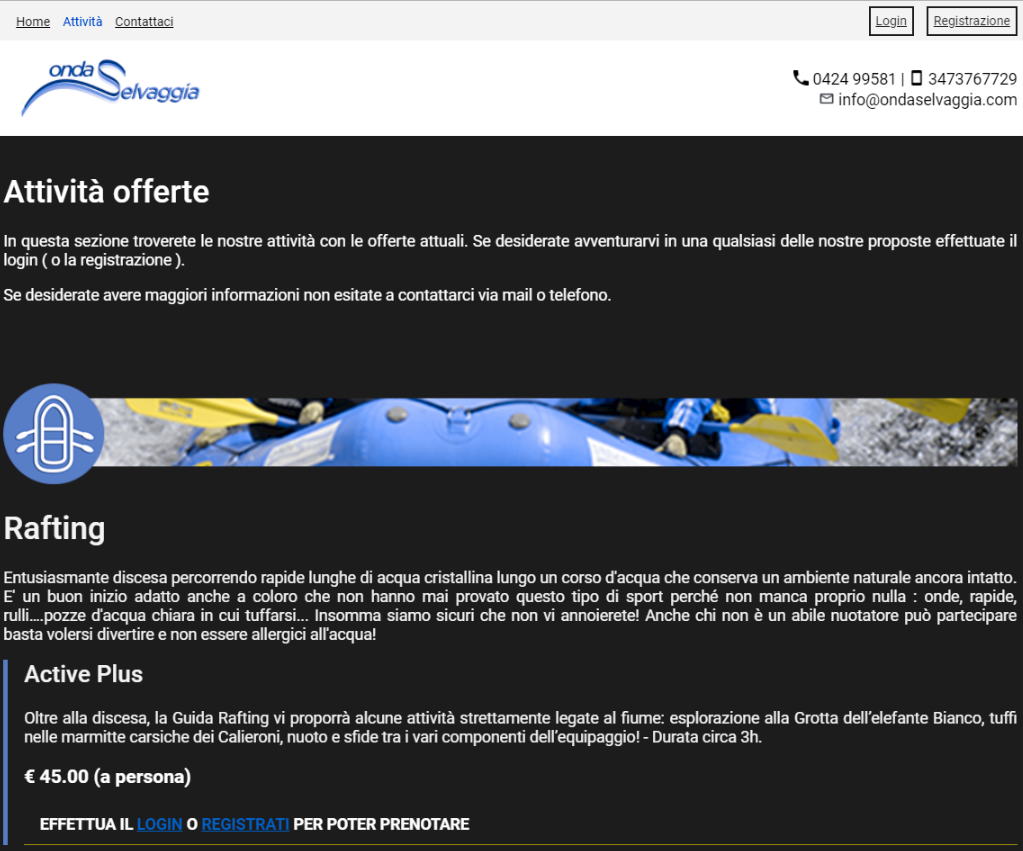
\includegraphics[scale=0.26]{images/deut.png}} \\
	\subfloat[][\emph{Protanopia}]
	{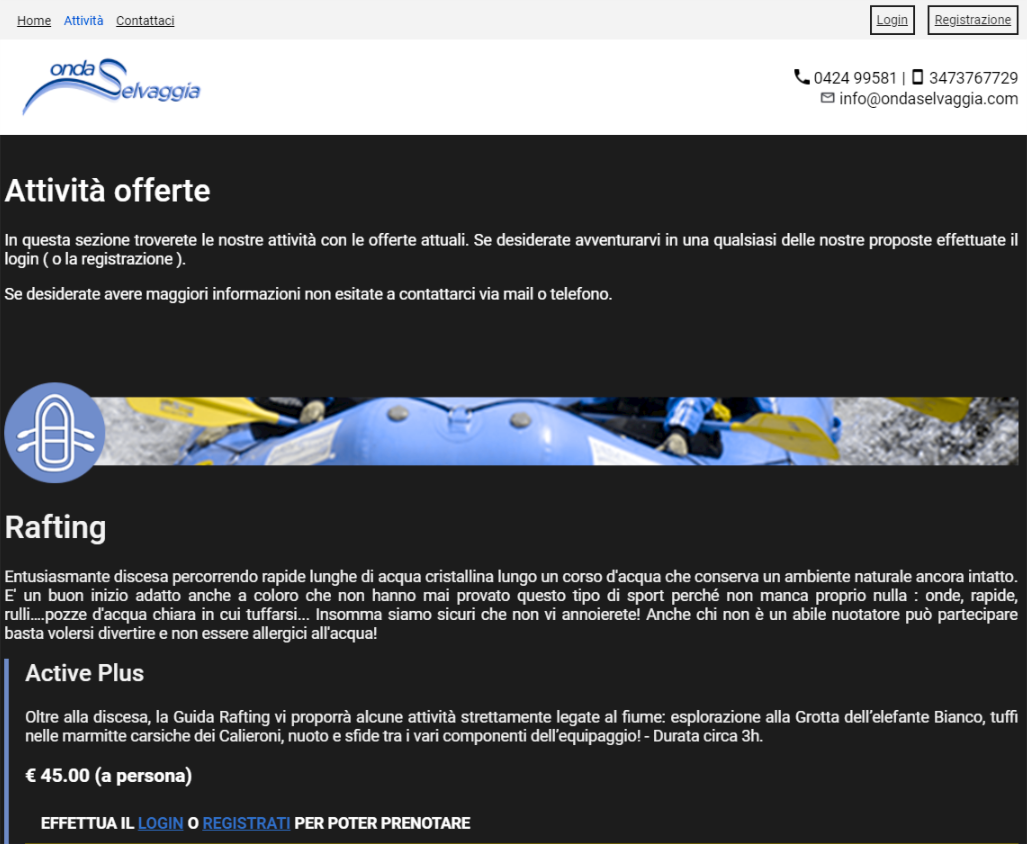
\includegraphics[scale=0.26]{images/tren.png}} \quad
	\subfloat[][\emph{Tritanopia}]
	{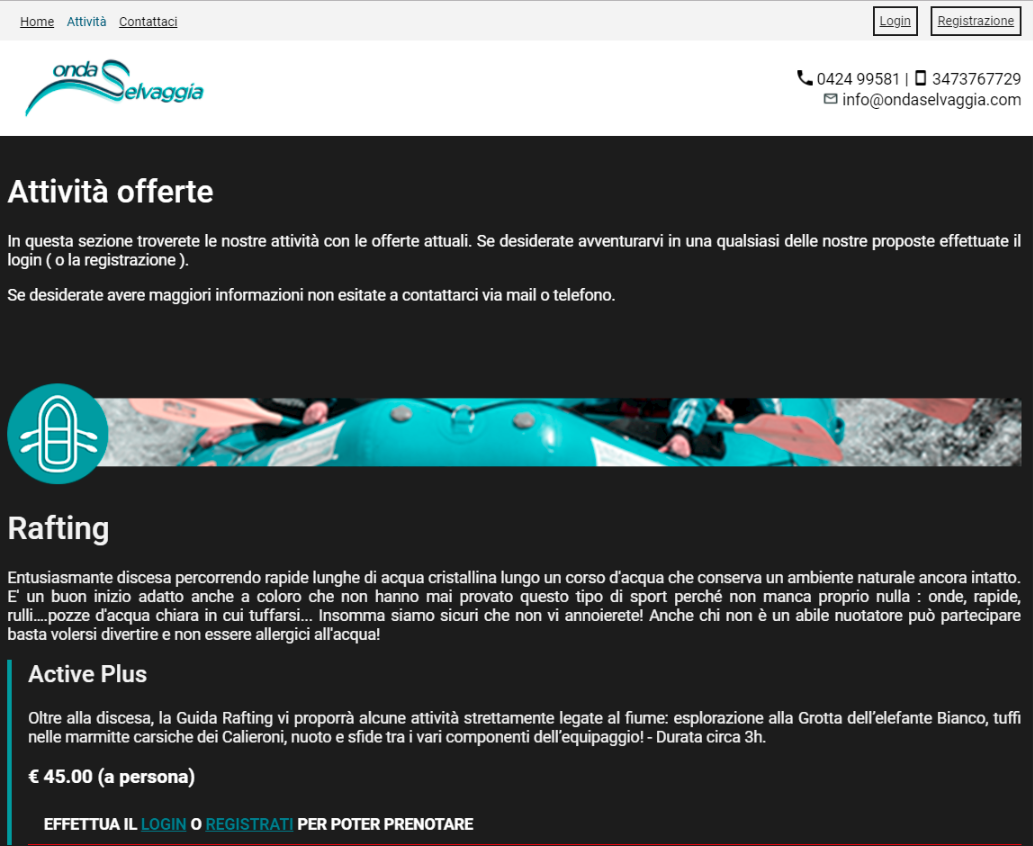
\includegraphics[scale=0.26]{images/tritano.png}} \\
	\caption{Simulazione di daltonismo della pagina Attivit�}
\end{figure}
\subsection{Contenuto, presentazione e comportamento}
Secondo i criteri standard si ha completa tra contenuto, presentazione e comportamento. [da continuare e specificare meglio]
\subsection{Tag}
Per quanto concerne i tag che migliorano l'accessibilit� si ha:
\begin{itemize}
 	\item Sono stati utilizzati in modo corretto i tag \texttt{alt} per le immagini.
 	\item Le parole in lingua inglese sono state racchiuse in un tag \texttt{<span lang="en"></span>} cos� da poter garantire una lettura corretta da parte degli screen-reader.
 	\item Sono stati utilizzati i tag \texttt{tabindex} in modo da permettere la navigazione corretta del sito attraverso il tasto TAB. Inoltre poich� l'intestazione del sito si ripete per ogni pagina � stato introdotta una voce del men� non visibile \texttt{Salta intestazione} che permette allo screen reader di saltare la lettura dell'intestazione e passare direttamente al contenuto.
\end{itemize}
\paragraph{Tag WAI-ARIA}\mbox{}\\
Sono stati utilizzati dei tag introdotti dalle specifiche WAI-ARIA che permettono di migliorare l'accessibilit� per gli utenti che utilizzano uno screen-reader.\\

